
% \subsection{INSTITUTIONAL SHIFTS AND STRUCTURES}
\section{流域社会\textendash{}生态系统的结构变迁}\label{results-1}

\begin{figure}[!ht]
	\includegraphics[width=\linewidth]{img/ch5/ch5_diagram.png}
	\caption[黄河流域社会\textendash{}生态系统的分水制度结构及其变迁]{
		黄河流域社会\textendash{}生态系统的分水制度结构及其变迁。
		\textbf{A} 黄河流域跨越$10$个省(地区),其中$8$个对黄河流域水资源的依赖程度较高。国家部委(水利部)是发布水治理政策的最高权力机构,这些政策通常由流域级机构黄河水利委员会和各省级机构执行。
		\textbf{B} 地方省政府(水利厅、局)是水分方案中的主要的利益相关者。自“八七”分水方案以来,由于黄河地表水的取用受到配额限制,利益相关者规划和利用水资源进行发展受到影响。自然水文过程是相互联系的,尽管配额制度主要限制地表水($Sur$),也可能通过社会水文过程影响流域内地下水($Gro$)或流域外地表水和地下水($Sur'$和$Gro'$)。
		\textbf{C} 制度变迁和随之而来的社会\textendash{}生态系统结构变化:
		(1) 1979 \textendash{} 1987年间,各利益相关方(红圈)从连接的生态单元(黄河河段,蓝圈)自由获取水资源。
		(2) 1987年施行“八七”分水方案后,黄河水利委员会(黄圈)负责监测各河段利益相关者用水情况。
		(3) 1998年施行“流域统一调度”之后,利益相关者必须向黄河水利委员会申请用水许可证(红黄圈之间的连接)。}\label{fig:structure}
\end{figure}

% 制度变动综述
1987年实施的“八七”分水方案和1998年实施的“流域统一调度”是黄河流域水治理中被广泛认可的里程碑事件。
在“八七”分水方案之前,参与分水方案的黄河流域各省份或地区可以根据其取水能力自由使用黄河的水资源进行开发,流域管理机构,即黄河水利委员会与这些地区在用水方面没有联系(图~\ref{fig:structure}~C)。
为缓解水资源压力,国家部委在“八七”分水方案中提出黄河流域$10$个省或地区之间应参照指定配额来取用水资源,且该配额与各省的预期取水量相去甚远(表~\ref{ch5:tab:quota})。
同时根据官方文件中的要求,黄河水利委员会需开始报告各省或地区和各个河段的用水情况。
这是黄河流域水利枢纽的责任首次涉及水资源利用,在社会与生态节点之间引入了新的联系(图~\ref{fig:structure}~C)。
由于备受争议的“八七”分水方案在此后十年内都没能解决黄河断流问题,1998年水利部签署同意了另一项制度变化——流域统一调度,强化了黄河水利委员会在综合管理用水方面的职责。
此次官方文件明确指出,各省须将其年度用水计划向黄河水利委员会报备并申请用水许可证,否则不再能使用黄河干流水资源,黄河水利委员会因此在社会\textendash{}生态系统结构中同各省直接联系在一起(图~\ref{fig:structure}~C)。
综上所述,两次制度转换重塑了黄河流域水资源利用的结构,形成的三类具一般性的社会\textendash{}生态系统结构块如图~\ref{fig:structure}~C所示。

% Table generated by Excel2LaTeX from sheet '八七分水方案配额'
\begin{table}[htbp]
    \caption{八七分水方案水资源配额}
      \begin{tabularx}{\textwidth}{p{2cm} LLLLLLLLLL}
      \toprule
            & \multicolumn{1}{l}{青海} & \multicolumn{1}{l}{四川$^b$} & \multicolumn{1}{l}{甘肃} & \multicolumn{1}{l}{宁夏} & \multicolumn{1}{l}{内蒙古} & \multicolumn{1}{l}{山西} & \multicolumn{1}{l}{陕西} & \multicolumn{1}{l}{河南} & \multicolumn{1}{l}{山东} & \multicolumn{1}{l}{津冀$^b$} \\
      \midrule
      规划需求  & 35.7  & 0     & 73.5  & 60.5  & 148.9 & 115   & 60.8  & 111.8 & 84    & 6 \\
      1983年方案 & 14    & 0     & 30    & 40    & 62    & 43    & 52    & 58    & 75    & 0 \\
      1987年方案 & 14.1  & 0.4   & 30.4  & 40    & 58.6  & 38    & 43.1  & 55.4  & 70    & 20 \\
      多年平均耗水$^a$ & 12.03 & 0.25  & 25.8  & 36.58 & 61.97 & 21.16 & 11.97 & 34.3  & 77.87 & 5.85 \\
      黄河水在地区总用水的占比 & 48.12\% & 0.10\% & 30.79\% & 58.45\% & 47.82\% & 73.55\% & 44.39\% & 24.77\% & 34.41\% & 3.11\% \\
      \bottomrule
      \end{tabularx}\label{ch5:tab:quota}%
      \footnotesize
      \\
      $a$ 使用1987年到2008年数据计算,四川因数据不足,使用2004到2017年数据计算。\\
      $b$ 由于取自黄河流域的水资源占省(或地区)总用水量的比值太小($< 5\%$),不在本研究中进行考虑。
\end{table}%


\section{制度变化对用水的影响}

\subsection{主成分提取结果}

具有解释力的变量是构建稳健的合成控制方法的关键。
本章使用了与用水相关的$24$个变量(见表~\ref{ch5:tab:data_source}),这些数据集在先前的研究中已用于解释中国用水的变化\cite{zhou2020};由于这些变量之间存在相关性,使用主成分分析进行降维并增强合成控制方法的稳健性。
研究发现采用肘部法确定$5$个主成分时,能解释$89.63\%$的方差变异。
其中第一个主成分解释$51.6\%$的方差变化,第二个主成分解释$16.9\%$的方差变化。
这两个主成分是对区域用水量影响最大的两个轴,其余主成分对用水量的解释力均低于$10\%$。

% \begin{figure}[!ht]
%     \centering
%     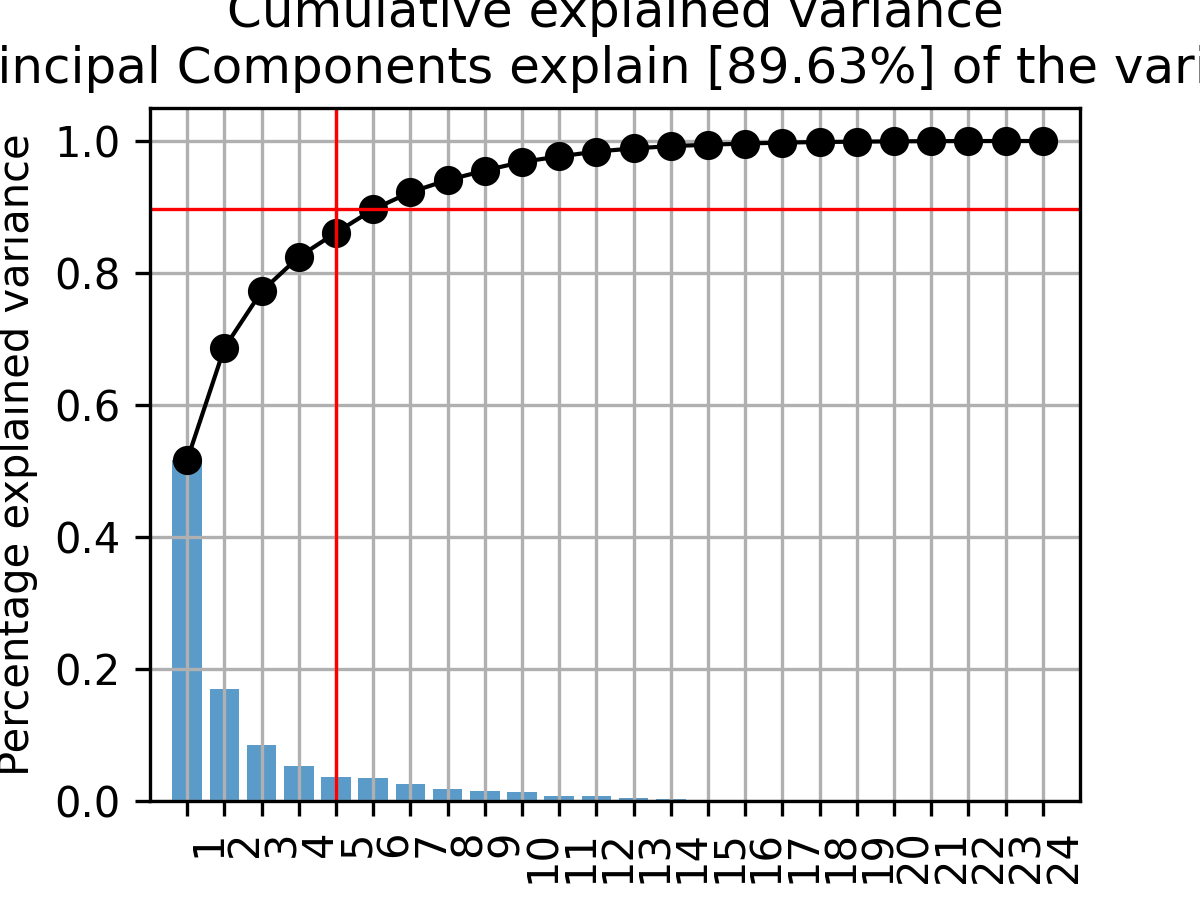
\includegraphics[width=0.6\textwidth]{img/ch5/ch5_elbow.png}
%     \caption{主成分分析的方差解释率肘部图}\label{ch5:fig:elbow}
% \end{figure}

使用双变量图同时展示数据集中样本点和变量特征,可以发现解释力最大的前$10$个特征大多和第一个主成分呈正相关(图\ref{ch5:fig:biplot})。
其中工业相关的自变量,如造纸、石化、纺织等高用水行业与第一个维度呈高度正相关;农业相关的自变量则仅呈现微弱正相关,但与第二个主成分呈高度相关(水稻正相关,小麦、玉米及其它农业负相关),可见主成分维度基本能够反映不同的区域的用水特征。
分析各特征在五个主成分上的负荷,可大致可将用水变量分为城市经济、农业灌溉、节水设施、气候适应、高耗水产业这五个类别(图~\ref{ch5:fig:variables})。


\begin{figure}[!ht]
    \centering
    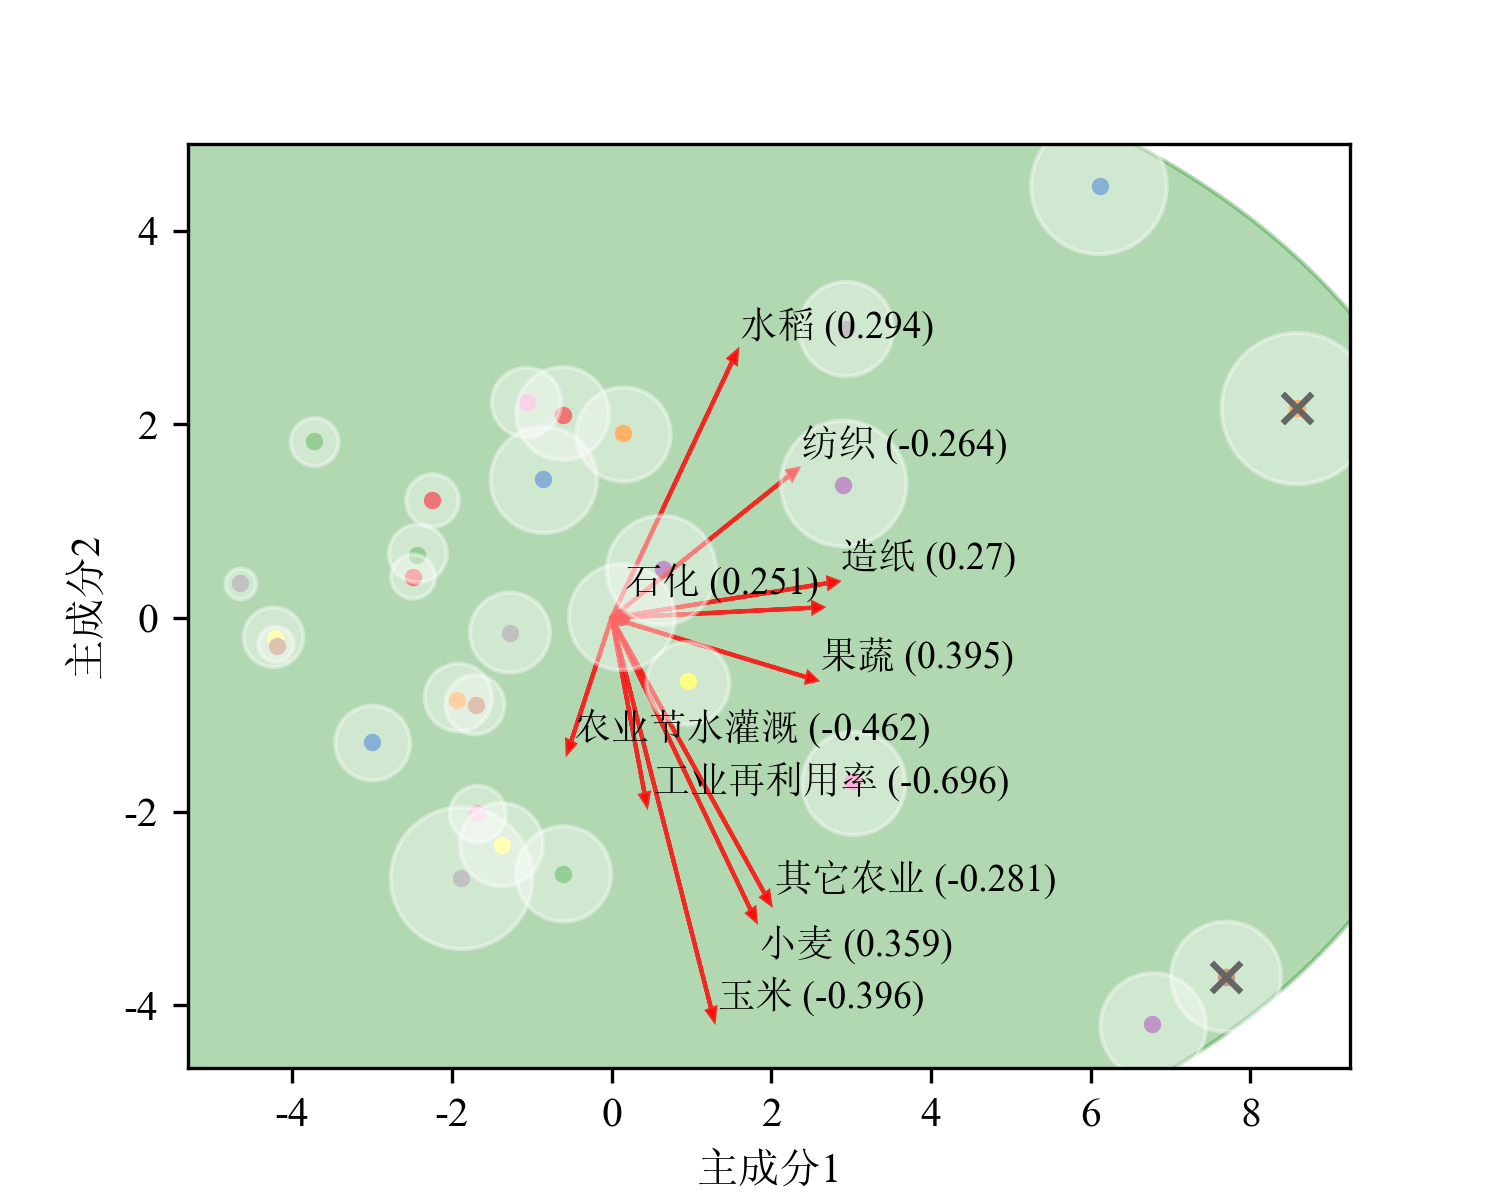
\includegraphics[width=0.6\textwidth]{img/ch5/ch5_biplot.png}
    \caption[主成分分析前两个主成分的双变量图]{主成分分析前两个主成分的双变量图(图中圆点为各省数据,x代表离群样本)}\label{ch5:fig:biplot}
\end{figure}


\begin{figure}[!ht]
    \centering
    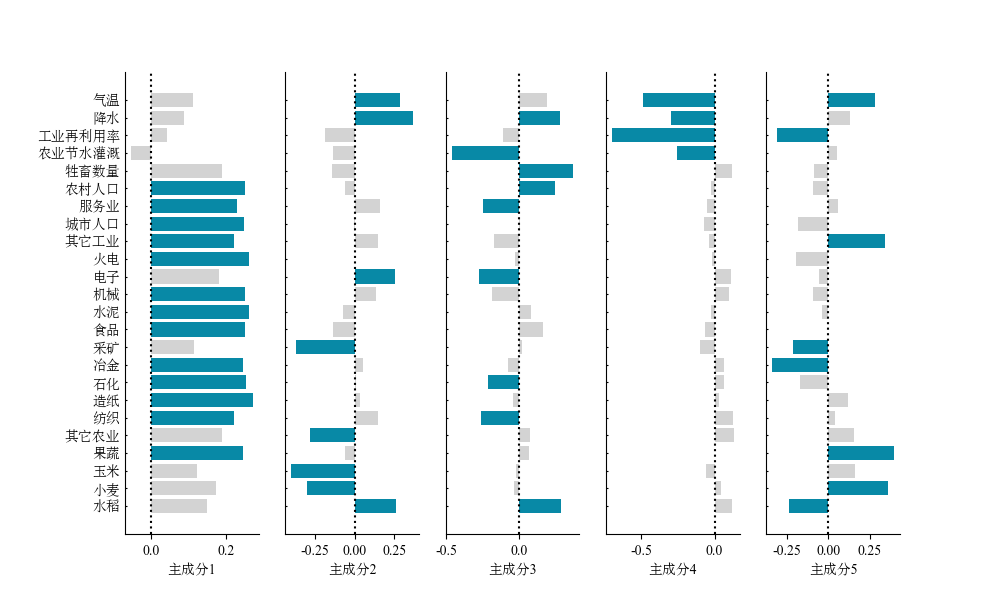
\includegraphics[width=\textwidth]{img/ch5/ch5_variables.png}
    \caption[区域用水量各主成分的特征显著性]{区域用水量各主成分的特征显著性(青色为该主成分中显著的变量)}\label{ch5:fig:variables}
\end{figure}

\subsection{合成控制结果}\label{result-2}
% 结果一:展示制度转变带来的用水量变化

黄河流域的总用水量在反事实推断模型和实际观测值在两次制度变化后呈现出差异显著,在之前此差异则较小且不显著(见图\ref{ch5:fig:main_results}A和B),这表明其用水变化的估计重建良好。
在1987年“八七”分水方案政策实施后,用水量变化速度的观测值为$1.82~km^3/yr$,比预测值$0.73~km^3/yr$高出$148.48\%$。
政策实施后$10$年间观测总用水量为$938.06$百万立方米,而预测值仅为$887.05$百万立方米,观测值比预测值高出$5.75\%$。
$T$检验结果显示在政策实施前,观测与预测之间用水量差异的$p$统计量为$0.93$,在政策实施后则下降至$0.003$,说明在政策实施前没有显著差异,但在政策实施后差异显著。
对用水量的理论估计表明,“八七”分水方案的制度转变促使各省取用了更多的水资源(图~\ref{ch5:fig:main_results}~A)

在1987年流域统一调度政策实施后,用水量的变化速度$-0.66~km^3/yr$,模型预测值则为$0.55~km^3/yr$,观测值比预测值低出两倍($-219.59\%$)。
在政策实施后的$9$年中(1998 \textendash{} 2008年),观测总用水量为$871.80$百万立方米,比预测值$931.08$百万立方米低$-6.37\%$。
$T$检验结果表明,政策实施前观测与预测间用水量差异的$p$统计量为$0.86$,在政策实施后为$0.002$。
同样说明在政策实施前没有显著差异,在政策政策实施后则差异显著。
可见在1998年流域统一调度制度出台后,用水量持续增加的趋势得到扭转(图~\ref{ch5:fig:main_results}~B)。

\begin{figure}[!ht]
	\centering
	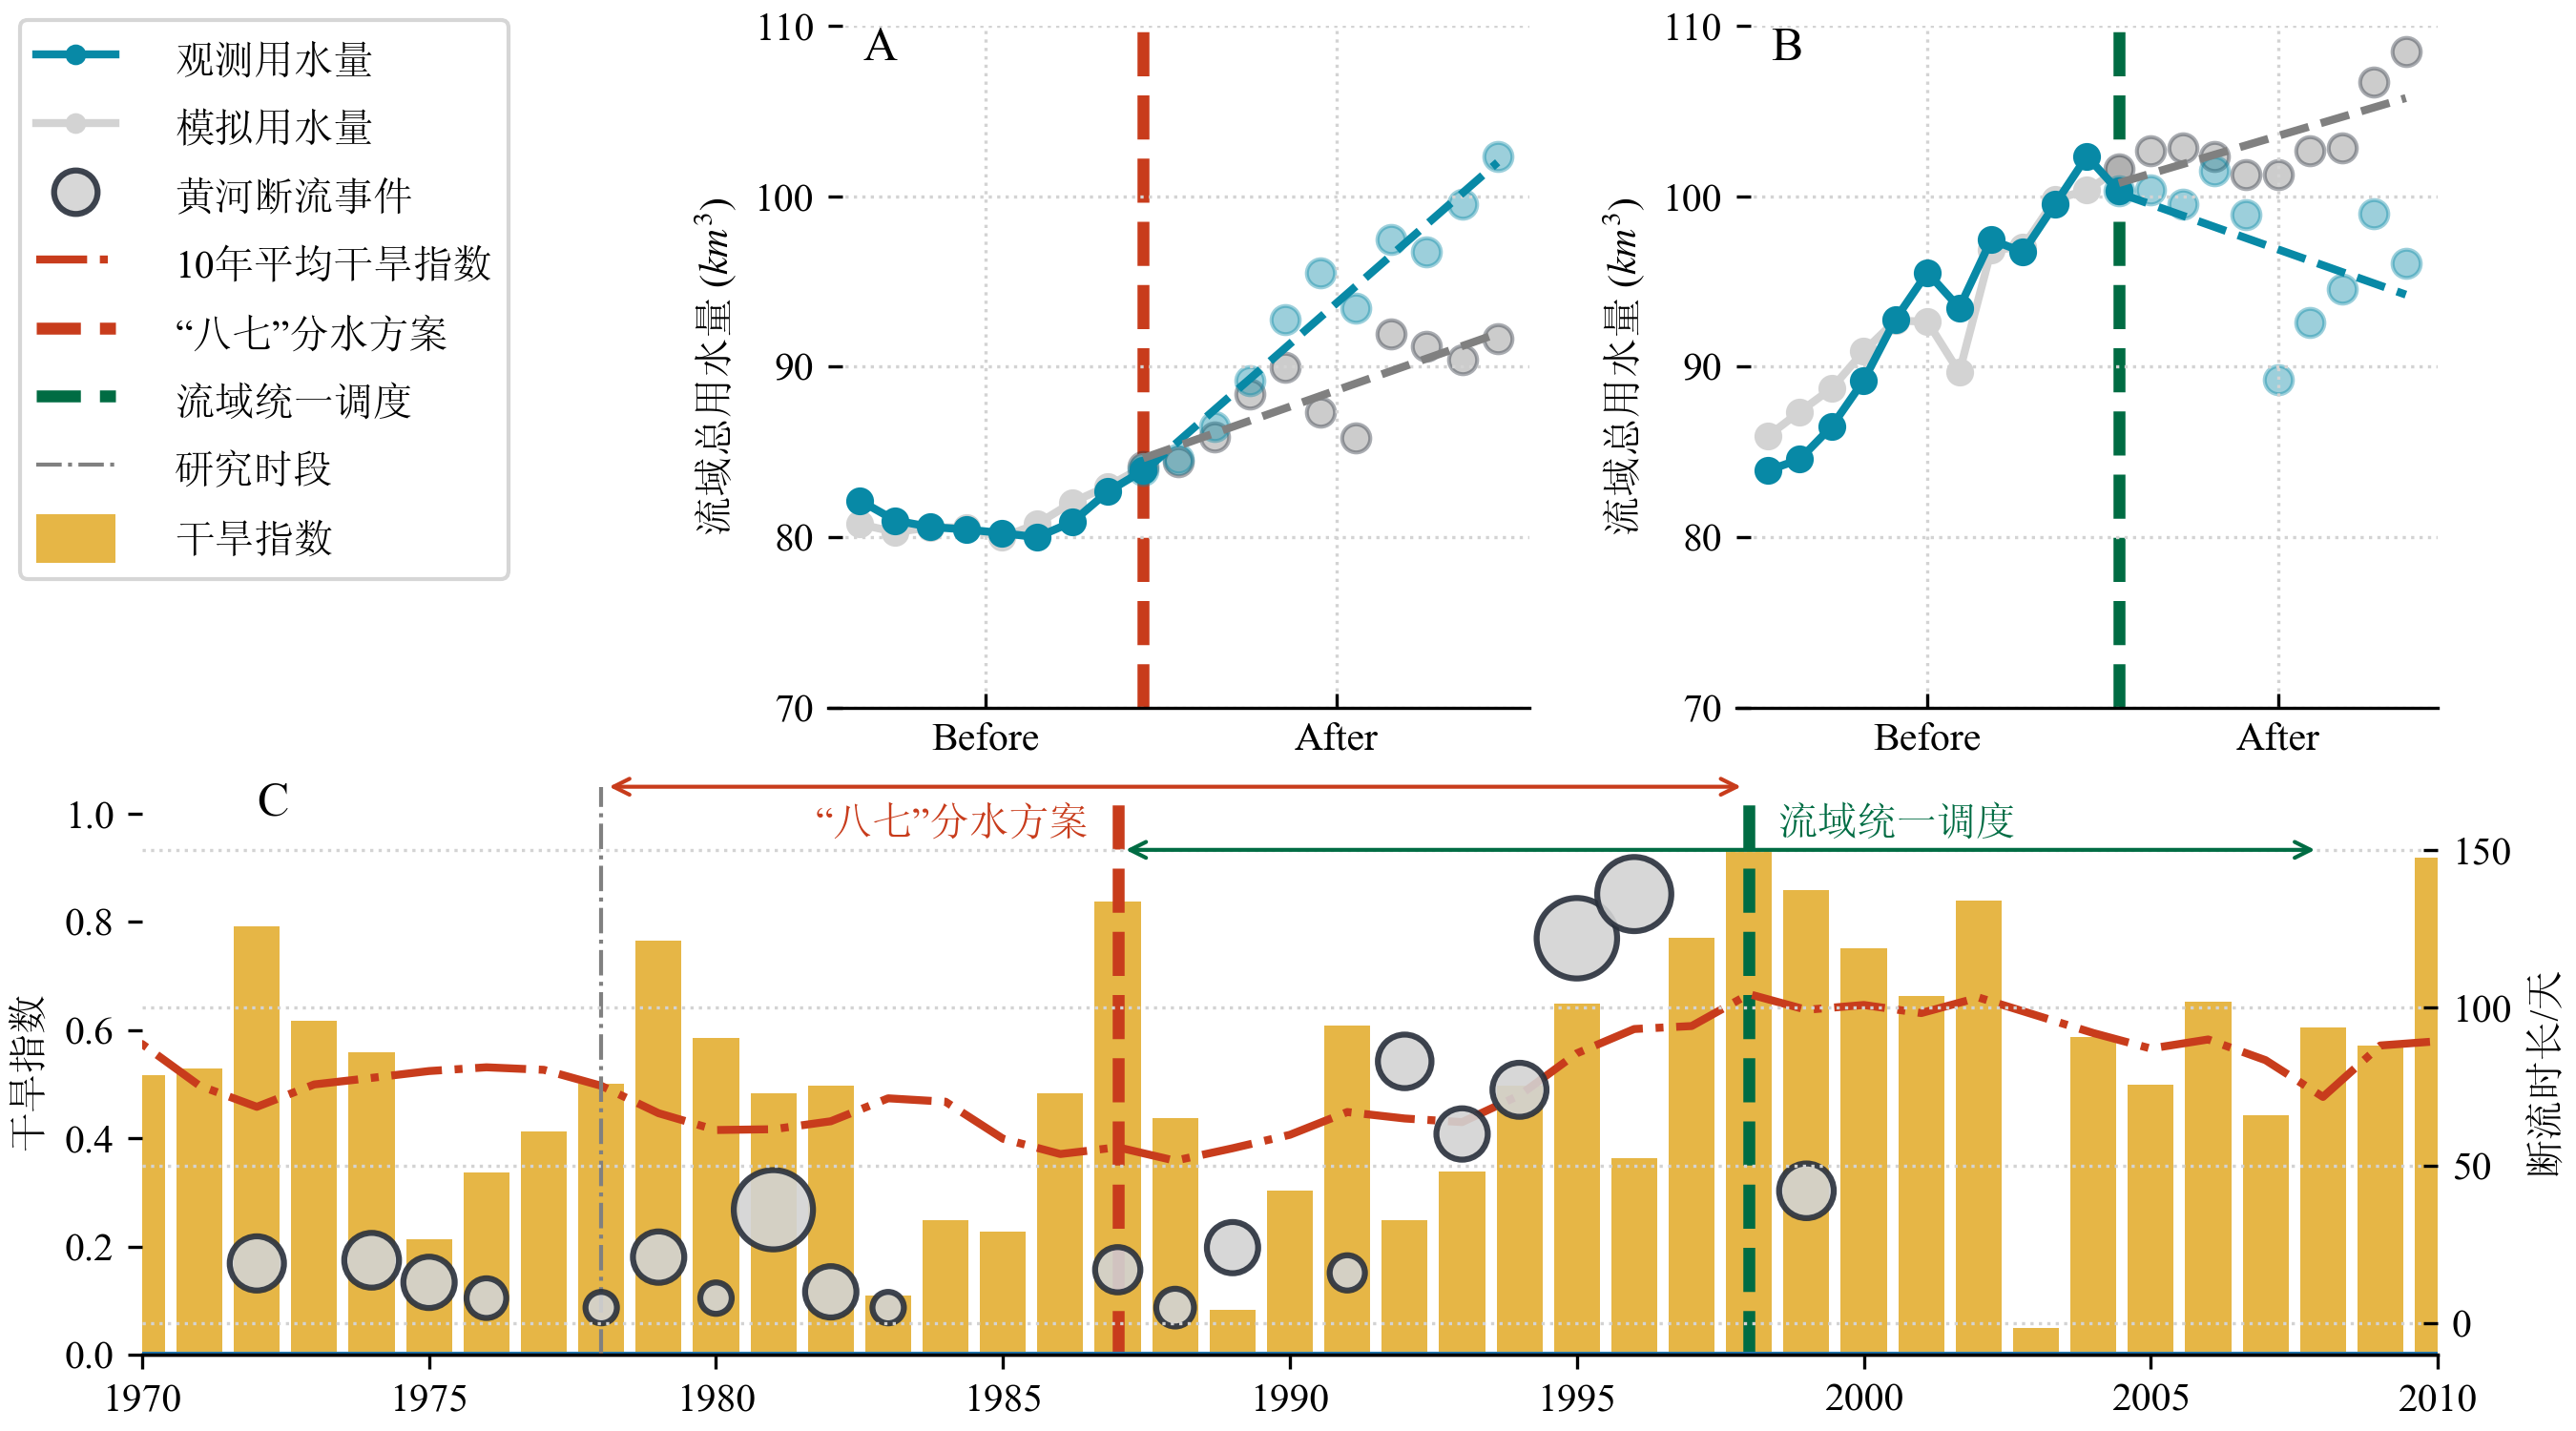
\includegraphics[width=\linewidth]{img/ch5/ch5_results.png}
	\caption[黄河流域两次水资源分配制度变化的影响]{
        黄河流域两次水资源分配制度变化的影响。
        \textbf{A} “八七”分水方案前后黄河流域用水量($1 \times 10^9~m^3$);
        \textbf{B} 流域统一调度前后黄河流域的用水情况。蓝线是来自统计资料的用水量,灰色线为经济和环境背景控制下差分合成控制法的估计值;
        \textbf{C} 黄河流域干旱强度与断流事件,灰色气泡的大小表示断流河段的长度。
	}\label{ch5:fig:main_results}
\end{figure}

“八七”分水方案后用水量的增加与1987 \textendash{} 1998年日益严重的黄河断流相一致,无论是断流时长还是断流河段长度都在此时期持续增加,导致流域生态退化危机(图~\ref{ch5:fig:main_results}~C)。
但在1987年流域统一调度之后,立竿见影地结束了长达二十余年的河流断流。
尽管1998 \textendash{} 2008年黄河流域的平均干旱强度高于1987 \textendash{} 1998年(平均干旱指数从$0.47$提升至$0.62$,图~\ref{ch5:fig:main_results}~C)。
这再一次证明了1987年提出“八七”分水方案最初没有有效限制用水,直到1998年的流域统一调度制度才成功限制了用水。

\subsection{鲁棒性检验}

对上述合成控制法拟合的结果进行鲁棒性检验,结果如表\ref{ch5:tab:RMSE}所示,柱状图长度代表政策实施后与政策实施前的均方根误差之比,该比值越高则说明合成控制法的效果越好。
黑色为该区域的合成控制结果,灰色为所有安慰剂对照组,红色区间则是所有安慰剂对照均值的$95\%$置信度区间,黑色柱状图高于该红色区间则说明该区域效果显著好于安慰剂对照,即有超$95\%$的把握说明政策干预对该区域的影响是明显的、且合成控制法有效模拟了此影响。
在1987年“八七”分水方案政策实施后,河南、甘肃、内蒙古自治区的合成控制效果显著高于其它安慰剂实验组($p < 0.05$),这说明分水方案对这三个省份的用水有着显著作用;山西、陕西显著低于其它控制对照组,其余省份均无显著差异,说明政策干预对这些地区没有明显效果。
在1987年流域统一调度政策实施后,除了河南和内蒙古自治区的合成控制效果显著低于安慰剂实验组外($p > 0.05$),其余省份都显著高于安慰剂实验组,这说明1987年的政策干预对河南与内蒙古的用水没有显著影响;其余省份均受到该制度的强烈干预,促使用水量减少。


% Table generated by Excel2LaTeX from sheet 'Sheet1'
\begin{table}[!htbp]\footnotesize
	\centering
	\caption[合成控制法的安慰剂检验结果]{各省经合成控制法处理后/处理前的均方根预测误差(RMSE)及其显著性}
	\begin{tabularx}{\textwidth}{XXXXXXX}
	  \toprule
			& \multicolumn{3}{c}{``八七''分水方案} & \multicolumn{3}{c}{流域统一调度} \\
  \cmidrule{2-7}    省份  & \multicolumn{1}{c}{处理后/处理前} & 较均值 & \multicolumn{1}{c}{差异显著性} & \multicolumn{1}{c}{处理后/处理前} & 较均值   & \multicolumn{1}{c}{差异显著性} \\
	  \midrule
	  青海 & 5.26  & =     & FALSE & 5.89  & >     & TRUE \\
	  甘肃 & 10.37  & >     & TRUE  & 9.55  & >     & TRUE \\
	  宁夏 & 5.81  & =     & FALSE & 6.83  & >     & TRUE \\
	  内蒙古 & 7.11  & >     & TRUE  & 1.60  & <     & TRUE \\
	  陕西 & 1.72  & <     & TRUE  & 5.60  & >     & TRUE \\
	  山西 & 3.05  & <     & TRUE  & 3.01  & >     & TRUE \\
	  河南 & 20.66  & >     & TRUE  & 1.18  & <     & TRUE \\
	  山东 & 4.54  & =     & FALSE & 4.14  & >     & TRUE \\
	  \bottomrule
	  \end{tabularx}%
	\label{ch5:tab:RMSE}%
\end{table}%


% \begin{figure}
%     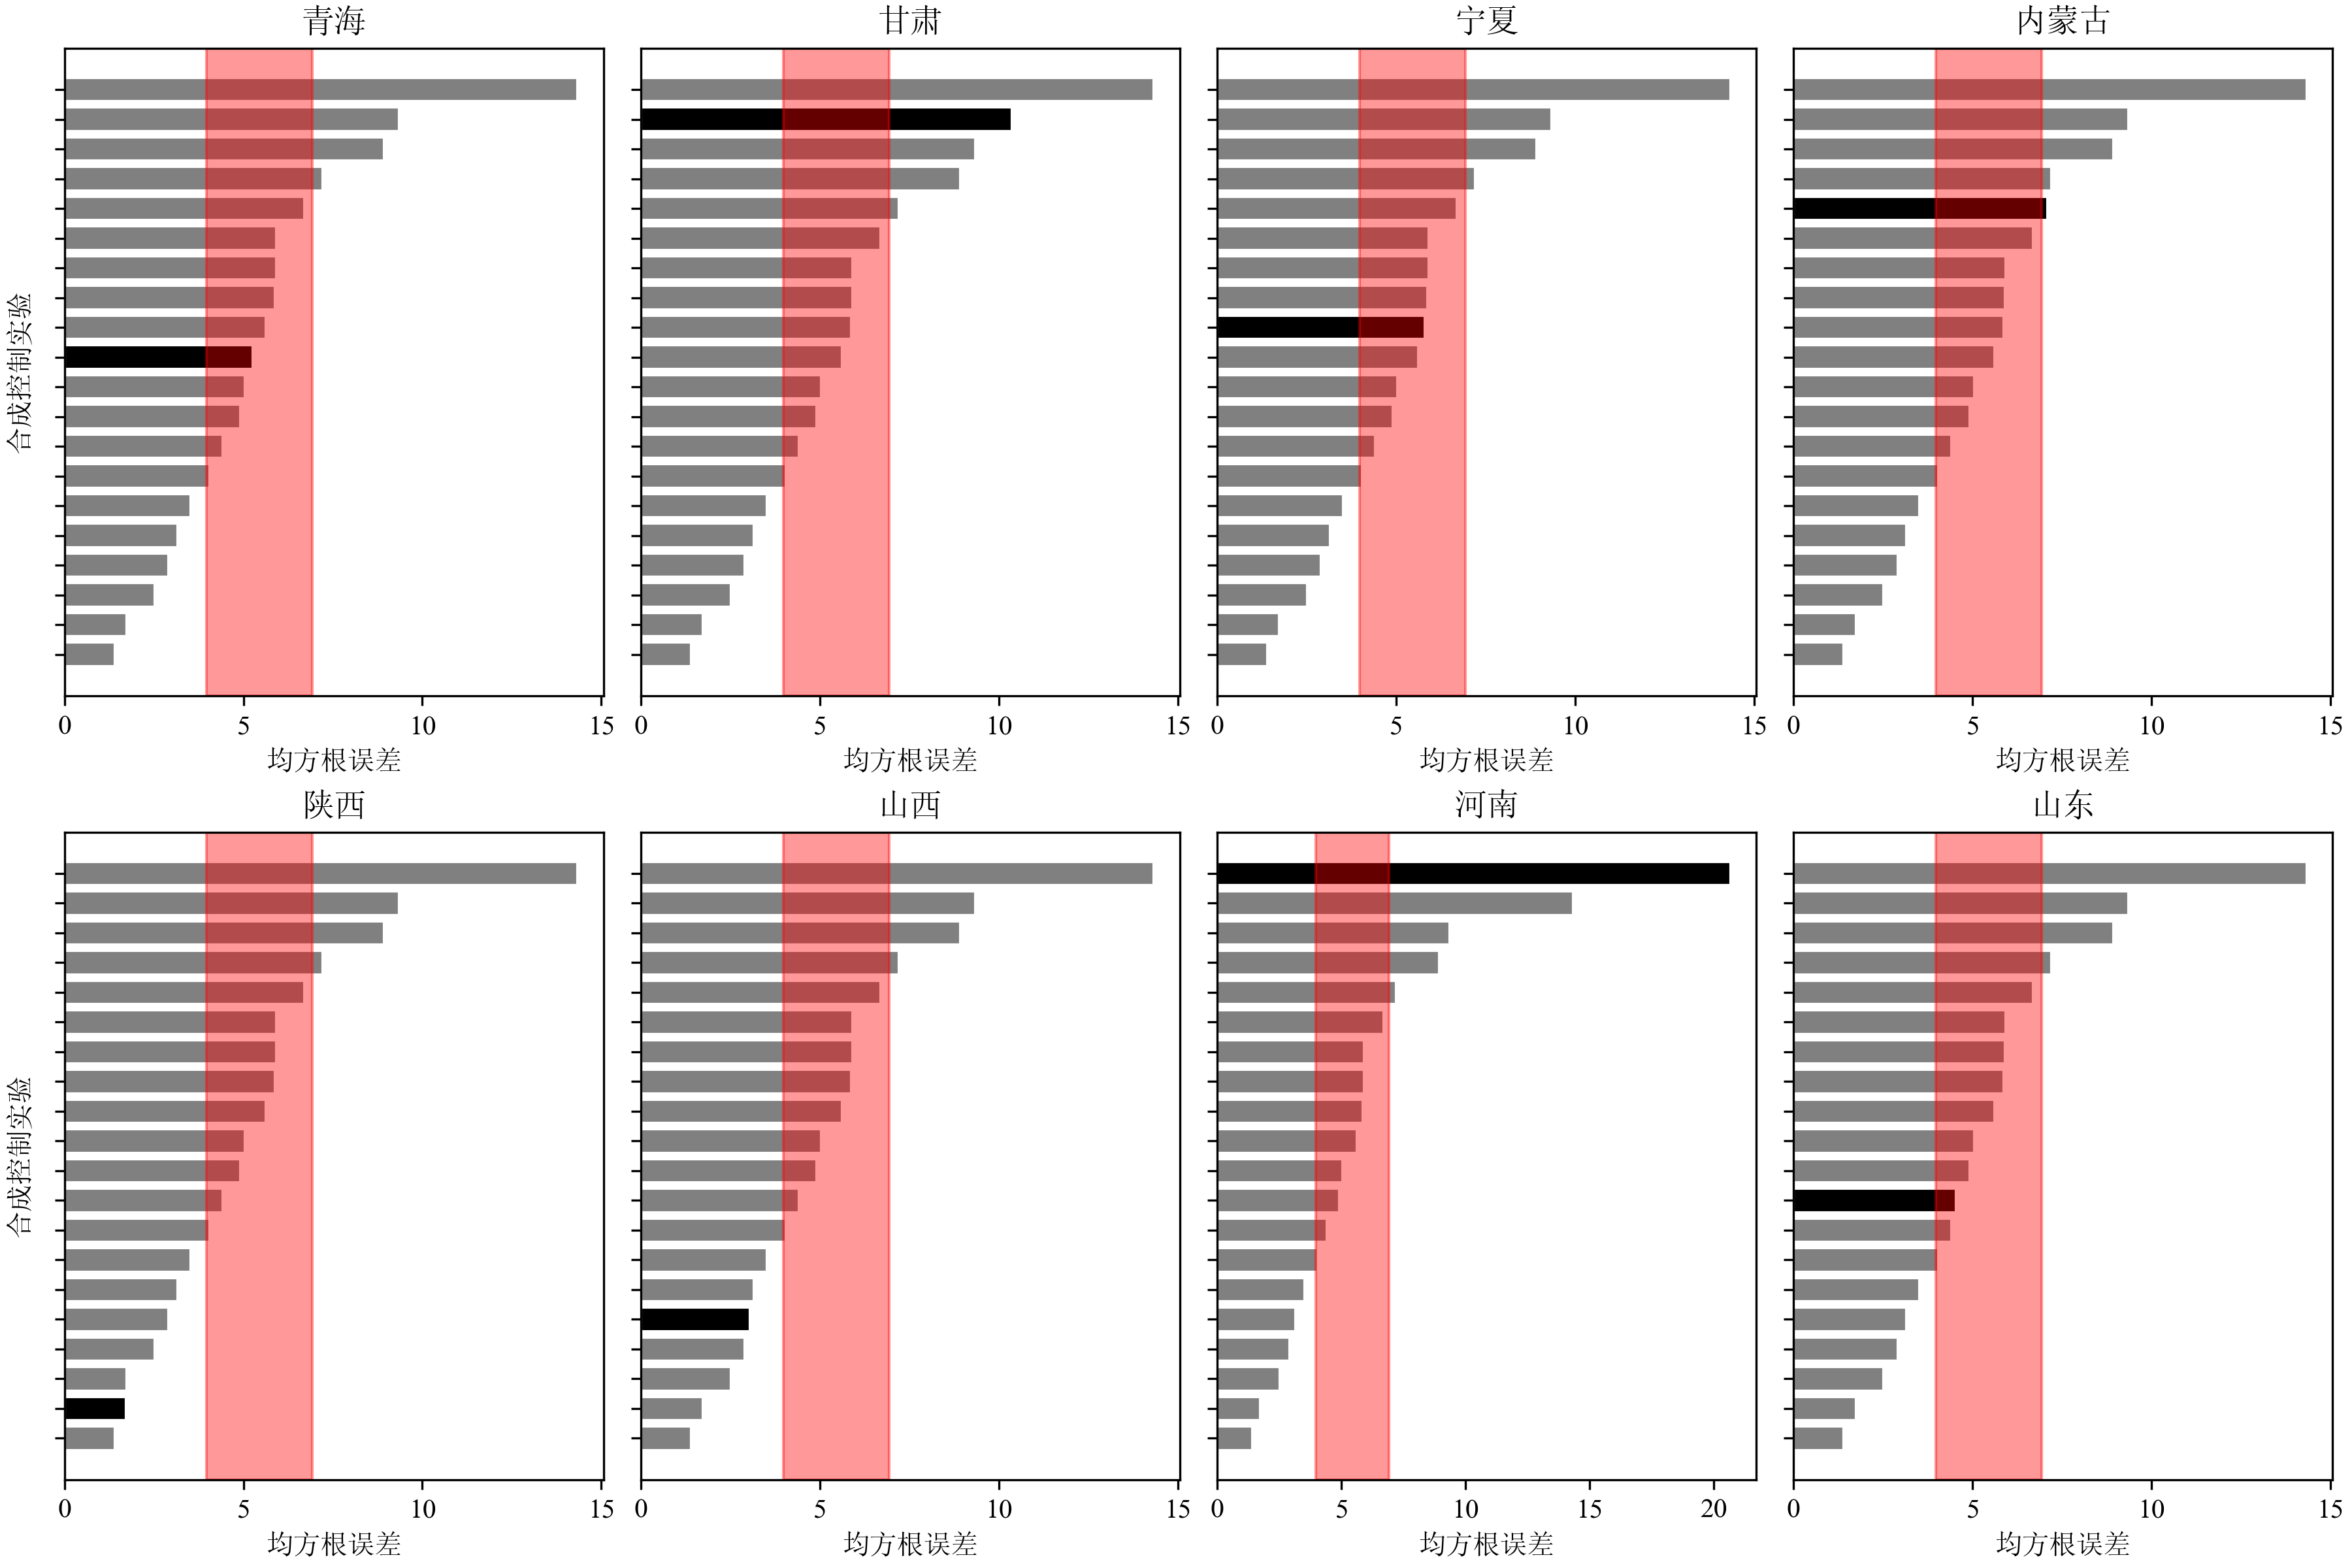
\includegraphics[width=0.9\linewidth]{img/ch5/ch5_rmse_87.png}
%     \centering
%     \caption[“八七”分水方案政策干预的安慰剂检验]{“八七”分水方案政策干预的安慰剂检验。深色柱子是当前省份的实验后/前均方根误差之比,灰色柱子是对所有非黄河流域其他省份构建合成控制模型得到的均方根误差之比,红色是$95\%$置信区间。深色柱子若落在该区间内,则说明该省份的合成控制模型与流域外省份相比不具有显著差异。}\label{fig:87placebo}
% \end{figure}

% \begin{figure}
%     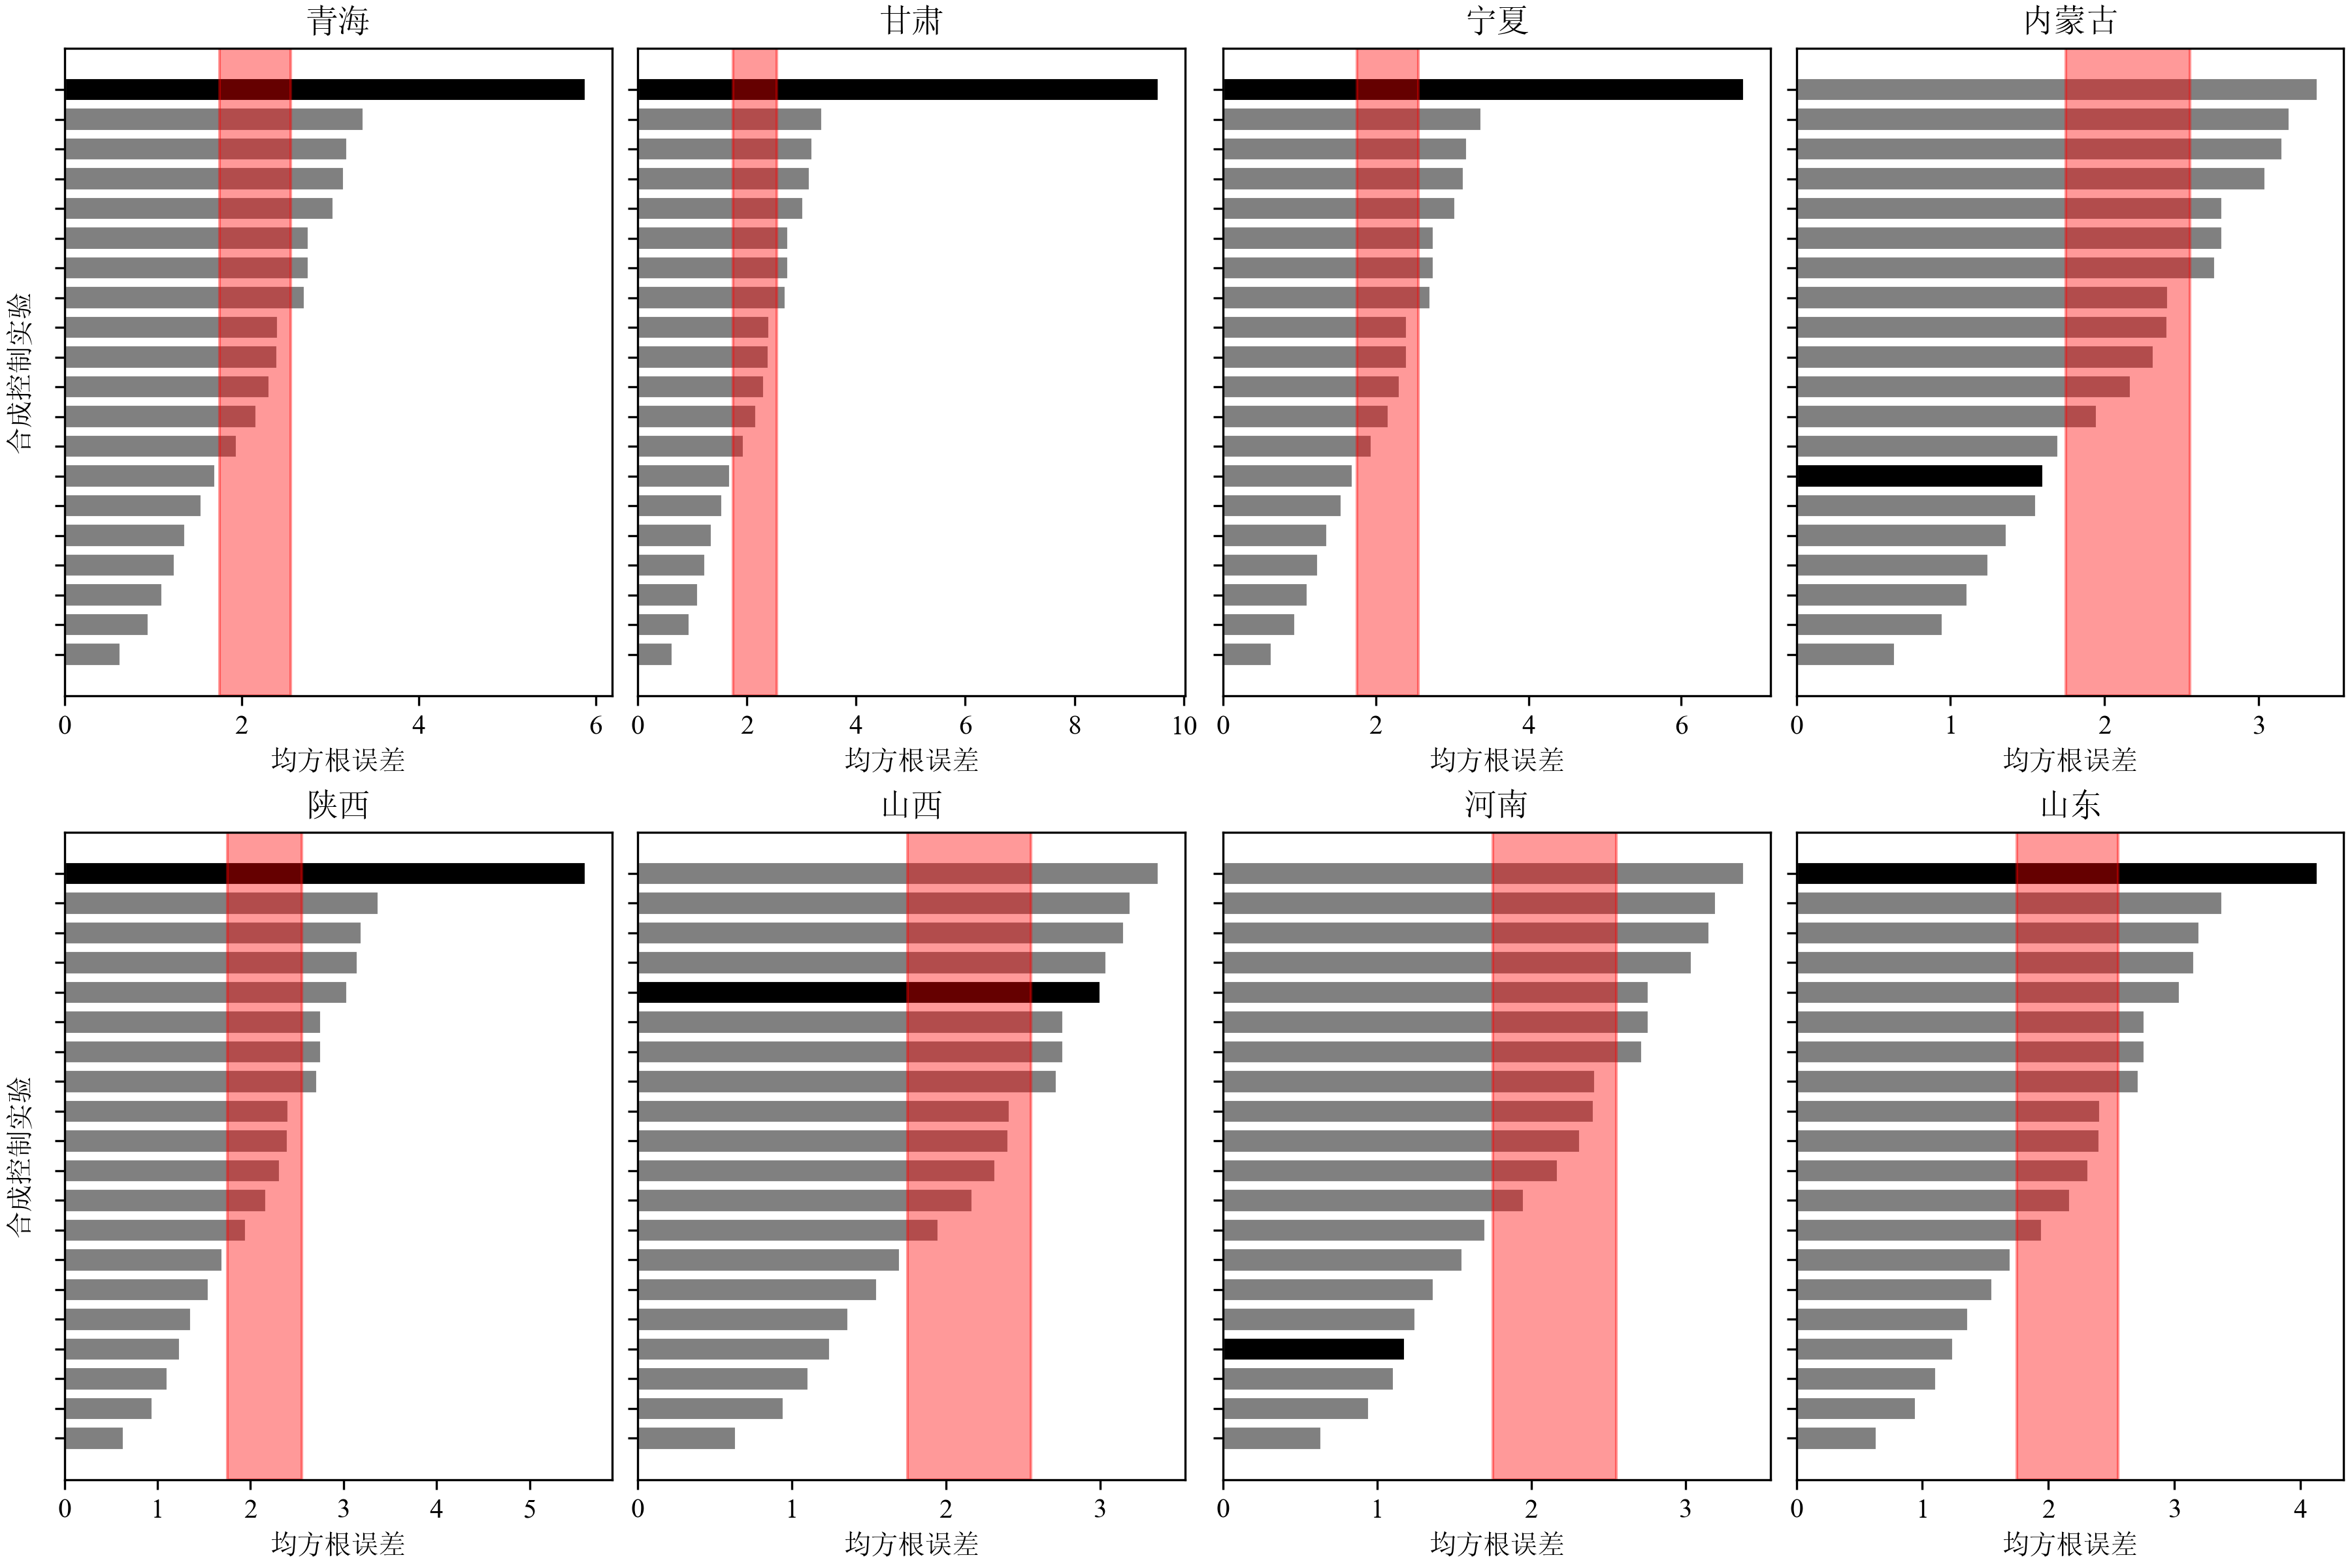
\includegraphics[width=0.9\linewidth]{img/ch5/ch5_rmse_98.png}
%     \centering
%     \caption[流域统一调度政策干预的安慰剂检验]{流域统一调度政策干预的安慰剂检验。深色柱子是当前省份的实验后/前均方根误差之比,灰色柱子是对所有非黄河流域其他省份构建合成控制模型得到的均方根误差之比,红色是$95\%$置信区间。深色柱子若落在该区间内,则说明该省份的合成控制模型与流域外省份相比不具有显著差异。}\label{fig:98placebo}
% \end{figure}


\subsection{各省的净效应差异}\label{result-3}

% 结果2部分:展示区域相应差异
研究结果表明各省(地区对这两次水资源分配制度变化的响应模式存在差异。
图\ref{fig:regulating}中,红色柱状图(“八七”分水方案)和绿色柱状图(流域统一调度)分别表示在该制度转变后的十年内,实际用水量相对于反事实推断模型估计值的增减比例;灰色柱状图显示了在两次制度转变后的十年内,各省实际用水量相对于其总用水量的比例;三角形标记指示“八七”分水方案为该省制定的理论水资源配额所占黄河流域总可用水量的比值。
在“八七”分水方案后的十年间,各省用水量相对反事实推断模型所估计用水量增加(或减少)的比例与其当前从黄河流域的取用水占比呈正相关(偏相关系数为$0.64$,图~\ref{fig:regulating})。
从1987年到1998年,一些用水大省(如内蒙古、河南、山东)也出现了显著的用水量增加(图~\ref{fig:regulating}),山东、内蒙古、河南和宁夏四省的用水量平均比预测值高出$32.14\%$。
而在施行流域统一调度后的1998年至2008年,几乎所有省份的用水量都出现了下降(平均下降$16.54\%$),
且各省用水量与从黄河流域的取用水占比变成了负相关(偏相关系数为$-0.51$)。

\begin{figure}[!ht]
	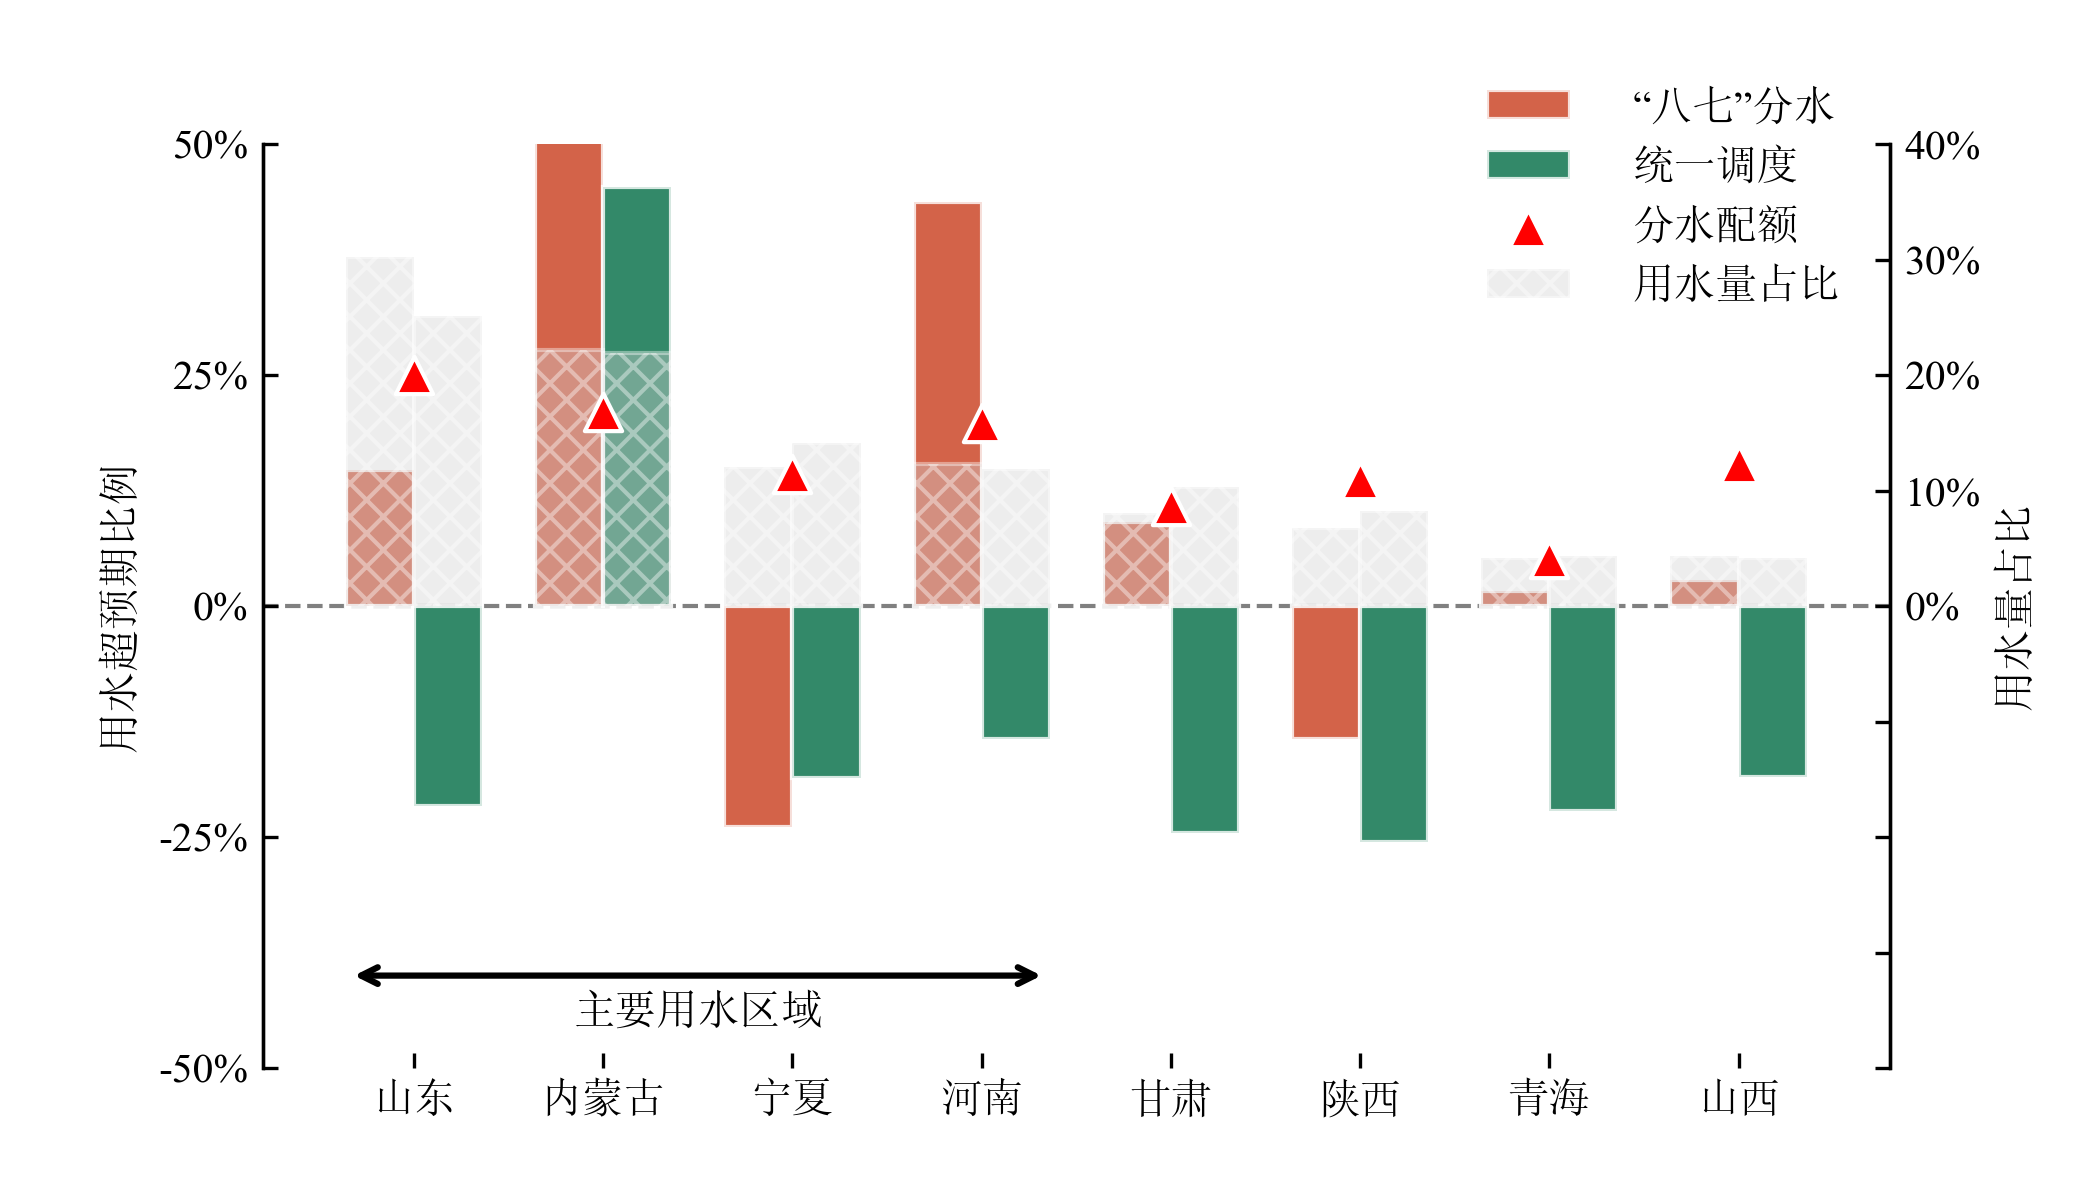
\includegraphics[width=\textwidth]{img/ch5/fig3.png}
	\caption[分水制度变化对黄河流域各省影响的差异]{分水制度变化对黄河流域各省影响的差异}\label{fig:regulating}
\end{figure}
